\documentclass[11pt]{article}
\usepackage[T1]{fontenc}
\usepackage[utf8]{inputenc}
\usepackage[a4paper,margin=2.2cm]{geometry}
\usepackage{amsmath,amssymb}
\usepackage{graphicx}
\usepackage{booktabs}
\usepackage{caption}
\usepackage[hidelinks]{hyperref}
\usepackage{xcolor}
\usepackage{authblk}
\usepackage{enumitem}
\captionsetup{font=small,labelfont=bf}
\definecolor{acc}{HTML}{C0562A}
\setlength{\parskip}{4pt}
\setlength{\parindent}{0pt}
\graphicspath{{figs/}}

\title{\textbf{Restoring Ankle Push-off Dynamics in Markerless Gait Analysis\\ by Calibrated Deconvolution}}
\author[1]{F.\ Fer}
\affil[1]{\small Institut de Myologie --- \texttt{myogait} technical report (proto-article)}
\date{August 2026}

\begin{document}
\maketitle
\vspace{-1.2em}

\begin{abstract}\noindent\small
Markerless two-dimensional pose estimation reproduces hip and knee sagittal kinematics well but systematically under-reads the ankle range of motion (ROM), chiefly by flattening the fast plantar-flexion of push-off. We show that, on a joint-angle waveform, the pose estimator behaves as a subject-independent low-pass filter: it retains about 80\% of the signal at 1\,Hz but only $\sim$20\% at 6--7\,Hz. Modelling the estimator as a linear time-invariant system with transfer function $H(f)$, we estimate $H$ once against synchronous optical motion capture (Vicon) on the BioCV dataset and invert it by Wiener deconvolution. The correction is applied as \emph{mean restoration}: because deconvolution is linear, the systematic deficit lives in the mean cycle whereas the cycle-to-cycle spread is the clinical variability signal that must be preserved; we therefore deconvolve only the mean and add the resulting per-phase correction to every cycle. In a leave-one-subject-out validation over 9 subjects and 85 walking trials, the ankle ROM bias is halved ($-10.6^\circ\!\to\!-5.3^\circ$), the absolute ROM error drops from $10.8^\circ$ to $6.7^\circ$, and inter-cycle variability is preserved exactly ($1.73^\circ$). The method requires no motion capture at run time, makes no healthy-gait assumption, and improves every subject.
\end{abstract}

\section{Introduction}
Optical marker-based motion capture is the clinical reference for joint kinematics but is costly, lab-bound and slow to set up. Video-based \emph{markerless} pipelines built on deep pose estimators---OpenPose~\cite{openpose}, and more recently high-resolution whole-body models such as Sapiens~\cite{sapiens}---promise the same measurement from a single camera~\cite{colyer2018}. Concurrent-validity studies now consistently report that hip and knee sagittal angles reproduce the optical reference to a few degrees, while the \emph{ankle} is the weakest joint~\cite{kanko2021,needham2021}. The dominant error is a flattened push-off: the real foot plantar-flexes sharply to propel the body, but the tracked foot landmarks do not follow that fast motion (Figure~\ref{fig:problem}).

Two families of remedies exist. Learned \emph{marker augmenters} map sparse video keypoints to dense anatomical markers using a network trained on motion capture, as in OpenCap~\cite{opencap}; parametric body-and-foot mesh models regularise the pose with a learned shape prior. Both are powerful but opaque and data-hungry. Here we ask whether a simple, interpretable, \emph{calibrated} signal-processing correction is enough. Our contributions are: (i) the observation that the estimator acts as a subject-independent low-pass filter on joint-angle waveforms; (ii) a cadence-adaptive Wiener deconvolution that inverts it from a filter calibrated once against Vicon; and (iii) a \emph{mean-restoration} scheme that recovers the systematic amplitude while leaving inter-cycle variability---itself a clinical marker~\cite{hausdorff2001}---mathematically unchanged. We also report, for completeness, a set of geometric multi-view reconstructions that were tried and did not solve the ankle (Appendix~\ref{app}).

\begin{figure}[t]\centering
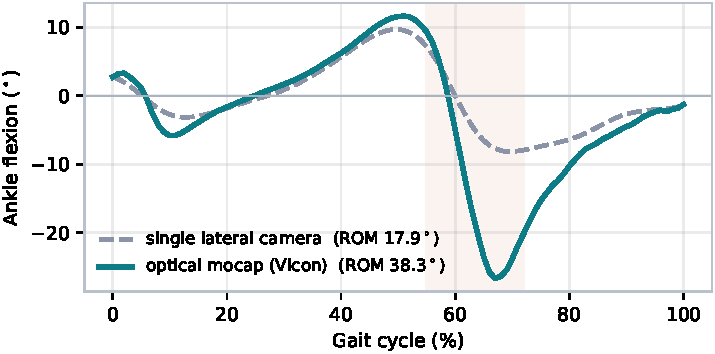
\includegraphics[width=0.82\linewidth]{fig1_problem.pdf}
\caption{The deficit (subject P06). During push-off (shaded, $\sim$55--72\% of the cycle) the optical reference reaches deep plantar-flexion, whereas the single lateral camera barely dips. The error is fast and phase-locked.}
\label{fig:problem}
\end{figure}

\section{Method}
\subsection{Data and angle extraction}
Video is processed by the \texttt{myogait} pipeline: per-axis normalisation, a 4\,Hz Butterworth filter, 2-D sagittal joint angles, coordinate-based (Zeni) event detection, and time normalisation of each gait cycle to 101 points. The optical reference is the Visual3D-processed Vicon of the same trial, from which we recompute the ankle from the full 3-D markers. All angles are compared after removing the whole-cycle mean, so a definition offset between the two systems does not bias the comparison.

\subsection{The pose estimator as a linear filter}
Write $c(\phi)$ for the true (Vicon) ankle angle over the normalised cycle $\phi$ and $v(\phi)$ for the markerless one. Taking the discrete Fourier transform over the cycle, the ratio between the video and reference spectra at each stride harmonic $k$ is, across subjects, a smooth and reproducible function of frequency that decays with $k$ (Figure~\ref{fig:tf}). We therefore model the estimator as a linear time-invariant system,
\begin{equation}
V(f) = H(f)\,C(f),
\end{equation}
where $H(f)$ is the complex transfer function of the tracker. Because $H$ is a property of the estimator, not of the subject, it is estimated once and re-used. We sample it at the eight lowest harmonics with a Wiener (minimum mean-square) estimator over the training subjects,
\begin{equation}
\hat H_k \;=\; \frac{\big\langle V_k\,\overline{C_k}\big\rangle}{\big\langle |C_k|^2\big\rangle}.
\end{equation}

\begin{figure}[t]\centering
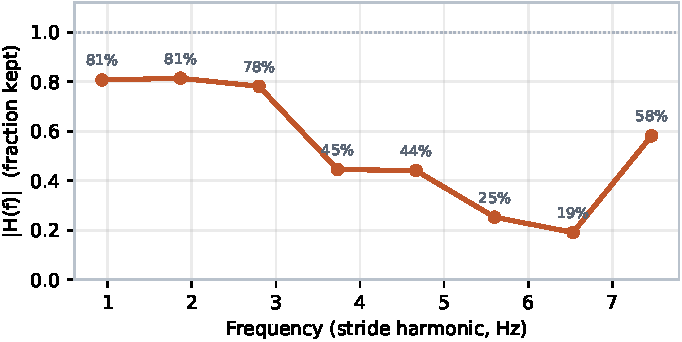
\includegraphics[width=0.74\linewidth]{fig2_transfer.pdf}
\caption{Estimated markerless transfer function $|H(f)|$: a low-pass. The tracker keeps $\sim$80\% of the ankle signal near 1\,Hz but only $\sim$20\% by 6--7\,Hz, exactly where the sharp push-off lives.}
\label{fig:tf}
\end{figure}

\subsection{Cadence-adaptive inversion}
At run time, for a trial of stride period $T$, harmonic $k$ sits at frequency $k/T$; we interpolate $H$ there, so the correction adapts to each subject's cadence and makes \emph{no} assumption about a healthy gait pattern. The waveform is restored by regularised (Wiener) inverse filtering,
\begin{equation}
\hat C_k \;=\; V_k\,\frac{\overline{H_k}}{|H_k|^2 + \lambda},\qquad \lambda = 0.08,
\end{equation}
the regulariser $\lambda$ trading restoration against noise amplification.

\subsection{Mean restoration}
Deconvolution amplifies high-frequency noise; applied to each raw cycle it would inflate the very inter-cycle variability we wish to measure. Because the deconvolution operator $\mathcal{D}$ is linear, $\operatorname{mean}(\mathcal{D}\{c_i\}) = \mathcal{D}\{\bar c\}$: the systematic deficit lives in the \emph{mean} cycle $\bar c$, while the deviations $c_i-\bar c$ carry the variability. We therefore deconvolve only the mean, form the per-phase correction, and add it to every cycle:
\begin{equation}
\Delta(\phi) = \mathcal{D}\{\bar c\}(\phi) - \bar c(\phi), \qquad
c_i^{\,\mathrm{corr}}(\phi) = c_i(\phi) + \Delta(\phi).
\end{equation}
Every cycle receives the \emph{same} correction $\Delta$, so the mean is restored to $\mathcal{D}\{\bar c\}$ while the cycle-to-cycle spread is left mathematically unchanged. This is the property that makes the method safe for variability-based clinical readings.

\subsection{Geometric reconstructions considered}
\label{sec:geom}
Before adopting deconvolution we tested whether the ankle deficit was \emph{geometric}---recoverable with additional calibrated cameras---rather than a limitation of the landmarks themselves. Two ingredients were combined.

\paragraph{Skeleton locking (rigid-body constraints).} Human segments are rigid. We first estimate each bone length as the temporal median $L_{ab}=\operatorname{median}_t\|X_a(t)-X_b(t)\|$ and rebuild the limb by chaining unit segment directions scaled by $L_{ab}$ from a triangulated pelvis root, so no frame can stretch or collapse a bone. The foot is treated as one rigid triangle (ankle--heel--toe): at each frame we fit the canonical foot template $\{p_j\}$ to the observed points $\{q_j\}$ by a rigid transform (a Procrustes / Kabsch solution),
\begin{equation}
(R^\star,t^\star)=\arg\min_{R\in SO(3),\,t}\sum_j \big\|R p_j + t - q_j\big\|^2,
\end{equation}
and read the foot orientation off $R^\star$. This removes the non-rigid jitter of the foot landmarks (their inter-marker distance was seen to vary by 20--26\% in video versus 2--5\% in Vicon), which cleans the ankle waveform (shape correlation with Vicon rose from $0.84$ to $0.88$) but does \emph{not} restore the missing amplitude.

\paragraph{Multi-view directional fusion.} A lateral camera constrains a segment's antero-posterior and vertical components but is nearly blind to depth; a near-orthogonal (frontal) camera constrains the complementary axis. For a segment 3-D direction $d$, each camera $c$ contributes one linear constraint: the observed 2-D direction $u_c$ must be parallel to $M_c\,d$, with $M_c$ the two in-plane rows of the camera rotation, i.e.\ $\big(u_c^{\perp\!\top} M_c\big)\,d = 0$. Two cameras give a $2\times3$ homogeneous system whose null space is $d$; chaining these directions with locked bone lengths yields a 3-D skeleton without triangulating the (noisy) foot position directly.

Both were evaluated but, as Appendix~\ref{app} shows, multi-view fusion \emph{degraded} the ankle relative to a single lateral view---the frontal camera tracks the foot poorly---so the reported method uses one lateral camera plus the calibrated deconvolution.

\section{Validation protocol}
We use the BioCV dataset (University of Bath Research Data Archive~\cite{biocv}): synchronous Sapiens-2 markerless video (lateral camera) and Visual3D Vicon, $9$ subjects, $85$ walking trials. The transfer function is estimated \textbf{leave-one-subject-out}: for each test subject $H$ is learned only on the others, so no test data enters the filter. Per trial and per side we report, for the ankle: the absolute ROM error and the signed bias versus Vicon; the waveform RMSE (mean-referenced); the inter-cycle SD (mean over phase of the standard deviation across a trial's cycles); and, across subjects, the inter-patient SD of the mean ROM. Agreement is summarised by Bland--Altman bias and $\pm1.96\,\mathrm{SD}$ limits of agreement (LoA).

\section{Results}
Figure~\ref{fig:curves} overlays, for three subjects, the raw and corrected mean cycle with their inter-cycle bands and the Vicon mean. The corrected curve deepens push-off toward the reference, and---crucially---the corrected band has the same width as the raw band. Table~\ref{tab:main} gives the pooled metrics: the ROM bias is halved and the absolute error drops by 38\%, while the inter-cycle SD is unchanged to two decimals. The Bland--Altman plots (Figure~\ref{fig:ba}) show the bias moving toward zero and the lower limit of agreement tightening. The correction improves \emph{every} subject (Figure~\ref{fig:persub}), and the between-subject spread of ankle ROM moves \emph{toward} the Vicon value ($3.6^\circ\!\to\!4.7^\circ$, Vicon $5.2^\circ$): real inter-patient differences are recovered, not smoothed away.

\begin{figure}[t]\centering
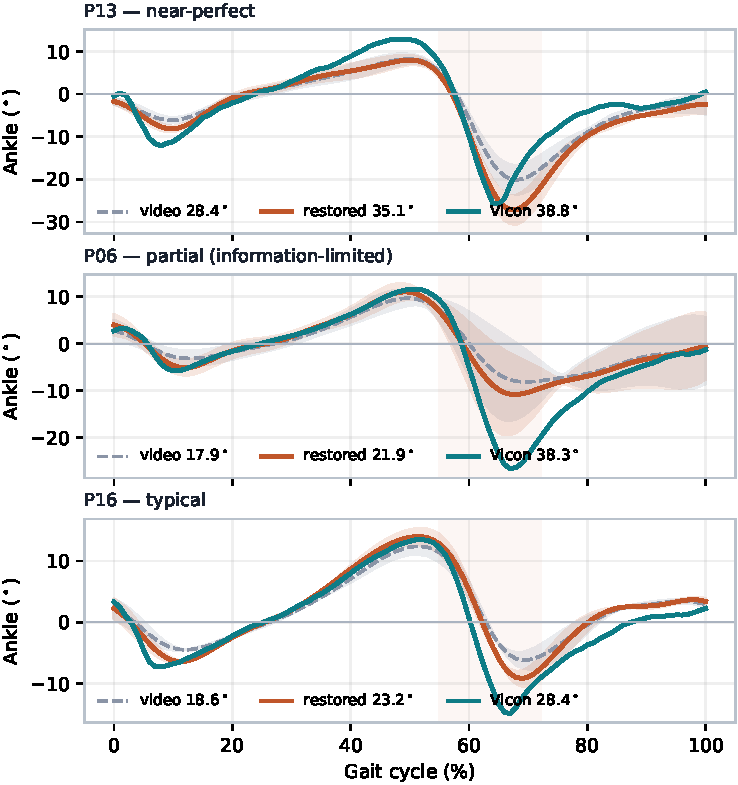
\includegraphics[width=0.72\linewidth]{fig3_curves.pdf}
\caption{Mean $\pm$ inter-cycle SD, three subjects. Raw video (grey, dashed), restored (orange), Vicon (teal). The corrected band width equals the raw band width---variability is preserved, not inflated.}
\label{fig:curves}
\end{figure}

\begin{table}[t]\centering\small
\caption{Ankle metrics, leave-one-subject-out ($9$ subjects, $85$ trials). Degrees.}
\label{tab:main}
\begin{tabular}{lcc}
\toprule
Metric (ankle) & Before & \textcolor{acc}{\textbf{After}} \\
\midrule
$|\text{ROM error}|$ vs Vicon      & 10.76 & \textcolor{acc}{\textbf{6.71}} \\
ROM bias (video $-$ Vicon)          & $-10.61$ & \textcolor{acc}{\textbf{$-5.29$}} \\
Waveform RMSE vs Vicon              & 3.70 & \textcolor{acc}{\textbf{3.43}} \\
Inter-cycle SD (preserved)          & 1.73 & \textcolor{acc}{\textbf{1.73}} \\
Inter-patient SD (Vicon $5.18$)     & 3.63 & 4.75 \\
\bottomrule
\end{tabular}
\end{table}

\begin{figure}[t]\centering
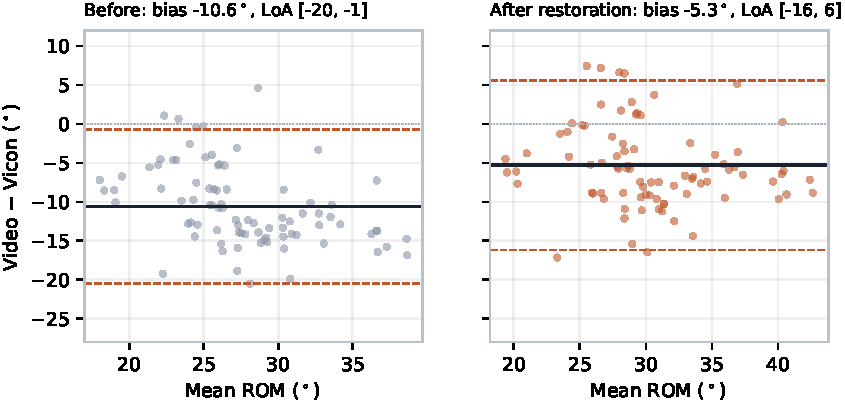
\includegraphics[width=0.92\linewidth]{fig4_bland_altman.pdf}
\caption{Bland--Altman on ankle ROM. The bias (solid) moves toward zero and the lower limit of agreement (dashed) tightens after restoration.}
\label{fig:ba}
\end{figure}

\begin{figure}[t]\centering
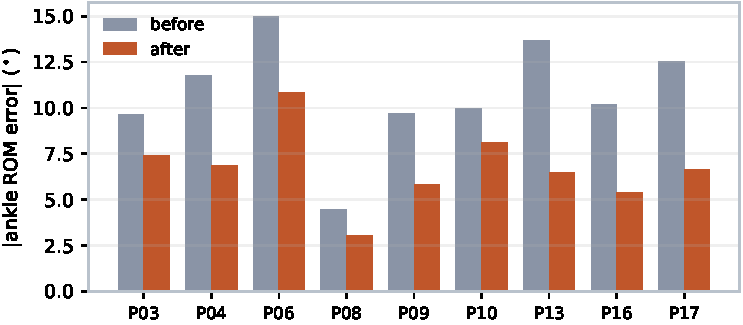
\includegraphics[width=0.72\linewidth]{fig5_persubject.pdf}
\caption{Per-subject absolute ankle ROM error, before and after. Every subject improves.}
\label{fig:persub}
\end{figure}

\section{Discussion}
The correction halves a systematic, phase-locked bias with a single lateral camera, one calibrated filter and about ten lines of code at run time. Three properties make it suitable for clinical, and specifically pathological, use. \emph{Variability is preserved} by construction, so gait variability is neither smoothed nor inflated. \emph{Inter-patient differences are restored, not erased}, which matters when the between-patient signal is itself the finding. And the filter is applied in Hz at the subject's own cadence, so there is \emph{no healthy-gait prior} that could hallucinate a normal pattern onto a pathological one. It generalises: leave-one-subject-out, all nine subjects improved.

\paragraph{Limitations.} (i) The residual bias ($\sim$5$^\circ$) is information the estimator never captured; a linear inverse filter can amplify what remains but cannot recreate what is absent---closing the gap further would require a learned non-linear augmenter~\cite{opencap}. (ii) The correction restores \emph{amplitude} (ROM); the point-wise RMSE improves only modestly, as some shape error persists. (iii) $H$ was estimated on one tracker and one dataset of healthy adults; a different tracker or population should re-estimate $H$ (the calibration, not the method, is specific). (iv) Multi-view fusion did not help the ankle (Appendix~\ref{app}), so a single lateral view plus this correction is the recommended configuration. A definitive clinical claim will require concurrent validation on a pathological cohort.

\section{Conclusion}
Treating a markerless pose estimator as a calibrated linear system and inverting it---while restoring only the systematic mean---recovers a clinically meaningful part of the ankle push-off that 2-D video loses, without motion capture at run time and without touching gait variability. The method ships in \texttt{myogait} as the opt-in \texttt{analyze\_gait(restore\_ankle\_dynamics=True)}.

\appendix
\section{Alternative reconstructions and ablation}
\label{app}
On the one subject with four calibrated views plus Vicon, we scored ten multi-view reconstruction strategies by mean absolute ROM error against Vicon (Figure~\ref{fig:alt}). Weighted or averaged fusion never beat the best single view; the strongest variant fused orthogonal image axes with locked bone lengths (Section~\ref{sec:geom}), yet even it plateaued, because the push-off is largely absent from the foot landmarks---no geometric method fully recovers it.

\begin{figure}[h]\centering
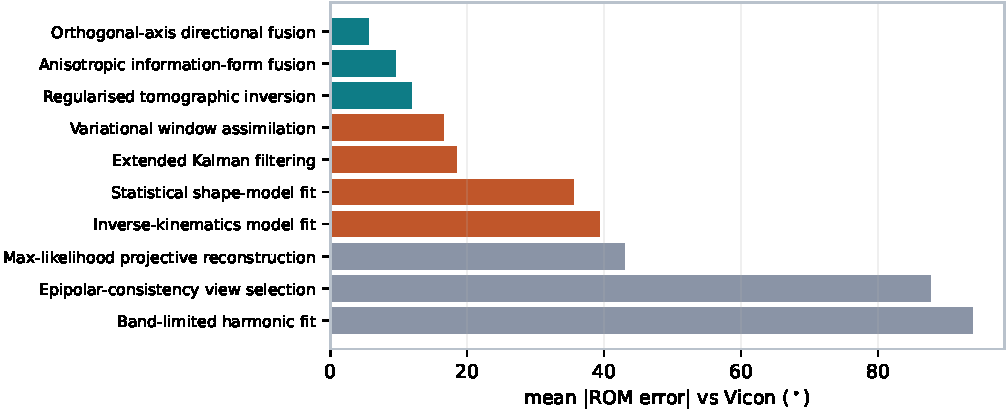
\includegraphics[width=0.78\linewidth]{fig6_alternatives.pdf}
\caption{Ten multi-view reconstruction strategies (subject P06), mean $|$ROM error$|$ vs Vicon. Teal: clear improvement (geometry-limited plateau); grey: failed.}
\label{fig:alt}
\end{figure}

The step-by-step ablation on the ankle (Table~\ref{tab:abl}) shows that deconvolution on a single lateral camera is the best single step; multi-camera fusion degrades the ankle and the methods do not stack. The raw per-cycle deconvolution used in this ablation inflates the inter-cycle SD; the mean-restoration variant of the main text removes that side-effect while keeping the accuracy gain.

\begin{table}[h]\centering\small
\caption{Ablation on the ankle (subject P06; Vicon ROM $\approx 38^\circ$). Degrees.}
\label{tab:abl}
\begin{tabular}{lccc}
\toprule
Configuration & ROM & RMSE & inter-cycle SD \\
\midrule
Single lateral camera & 24.7 & 4.40 & 4.71 \\
\textcolor{acc}{\textbf{\;+ deconvolution (this work)}} & \textcolor{acc}{\textbf{32.7}} & \textcolor{acc}{\textbf{3.37}} & \textcolor{acc}{\textbf{5.84}} \\
Multi-camera reconstruction & 20.8 & 5.80 & 5.70 \\
\;+ skeleton/foot locking & 20.0 & 5.77 & 5.34 \\
\;+ locking + deconvolution & 23.9 & 6.35 & 6.55 \\
\bottomrule
\end{tabular}
\end{table}

\begin{thebibliography}{9}\small
\bibitem{openpose} Z.~Cao, G.~Hidalgo, T.~Simon, S.-E.~Wei, Y.~Sheikh. OpenPose: Realtime multi-person 2D pose estimation using part affinity fields. \emph{IEEE TPAMI} 43(1):172--186, 2021.
\bibitem{sapiens} R.~Khirodkar, T.~Bagautdinov, J.~Martinez, et al. Sapiens: Foundation for human vision models. \emph{ECCV}, 2024.
\bibitem{colyer2018} S.~L.~Colyer, M.~Evans, D.~P.~Cosker, A.~I.~T.~Salo. A review of the evolution of vision-based motion analysis and the integration of advanced computer vision methods towards developing a markerless system. \emph{Sports Medicine -- Open} 4:24, 2018.
\bibitem{kanko2021} R.~M.~Kanko, E.~Laende, et al. Concurrent assessment of gait kinematics using marker-based and markerless motion capture. \emph{Journal of Biomechanics} 127:110665, 2021.
\bibitem{needham2021} L.~Needham, M.~Evans, D.~P.~Cosker, et al. The accuracy of several pose estimation methods for 3D joint centre localisation. \emph{Scientific Reports} 11:20673, 2021.
\bibitem{opencap} S.~D.~Uhlrich, A.~Falisse, \L.~Kidzi\'nski, et al. OpenCap: Human movement dynamics from smartphone videos. \emph{PLoS Computational Biology} 19(10):e1011462, 2023.
\bibitem{hausdorff2001} J.~M.~Hausdorff, D.~A.~Rios, H.~K.~Edelberg. Gait variability and fall risk in community-living older adults. \emph{Archives of Physical Medicine and Rehabilitation} 82(8):1050--1056, 2001.
\bibitem{winter2009} D.~A.~Winter. \emph{Biomechanics and Motor Control of Human Movement}, 4th ed. Wiley, 2009.
\bibitem{biocv} M.~Evans, L.~Needham, S.~Colyer, et al. BioCV dataset. University of Bath Research Data Archive, \href{https://doi.org/10.15125/BATH-01258}{doi:10.15125/BATH-01258}.
\end{thebibliography}

\end{document}
